\begin{figure}%[!htb] 
\centering 
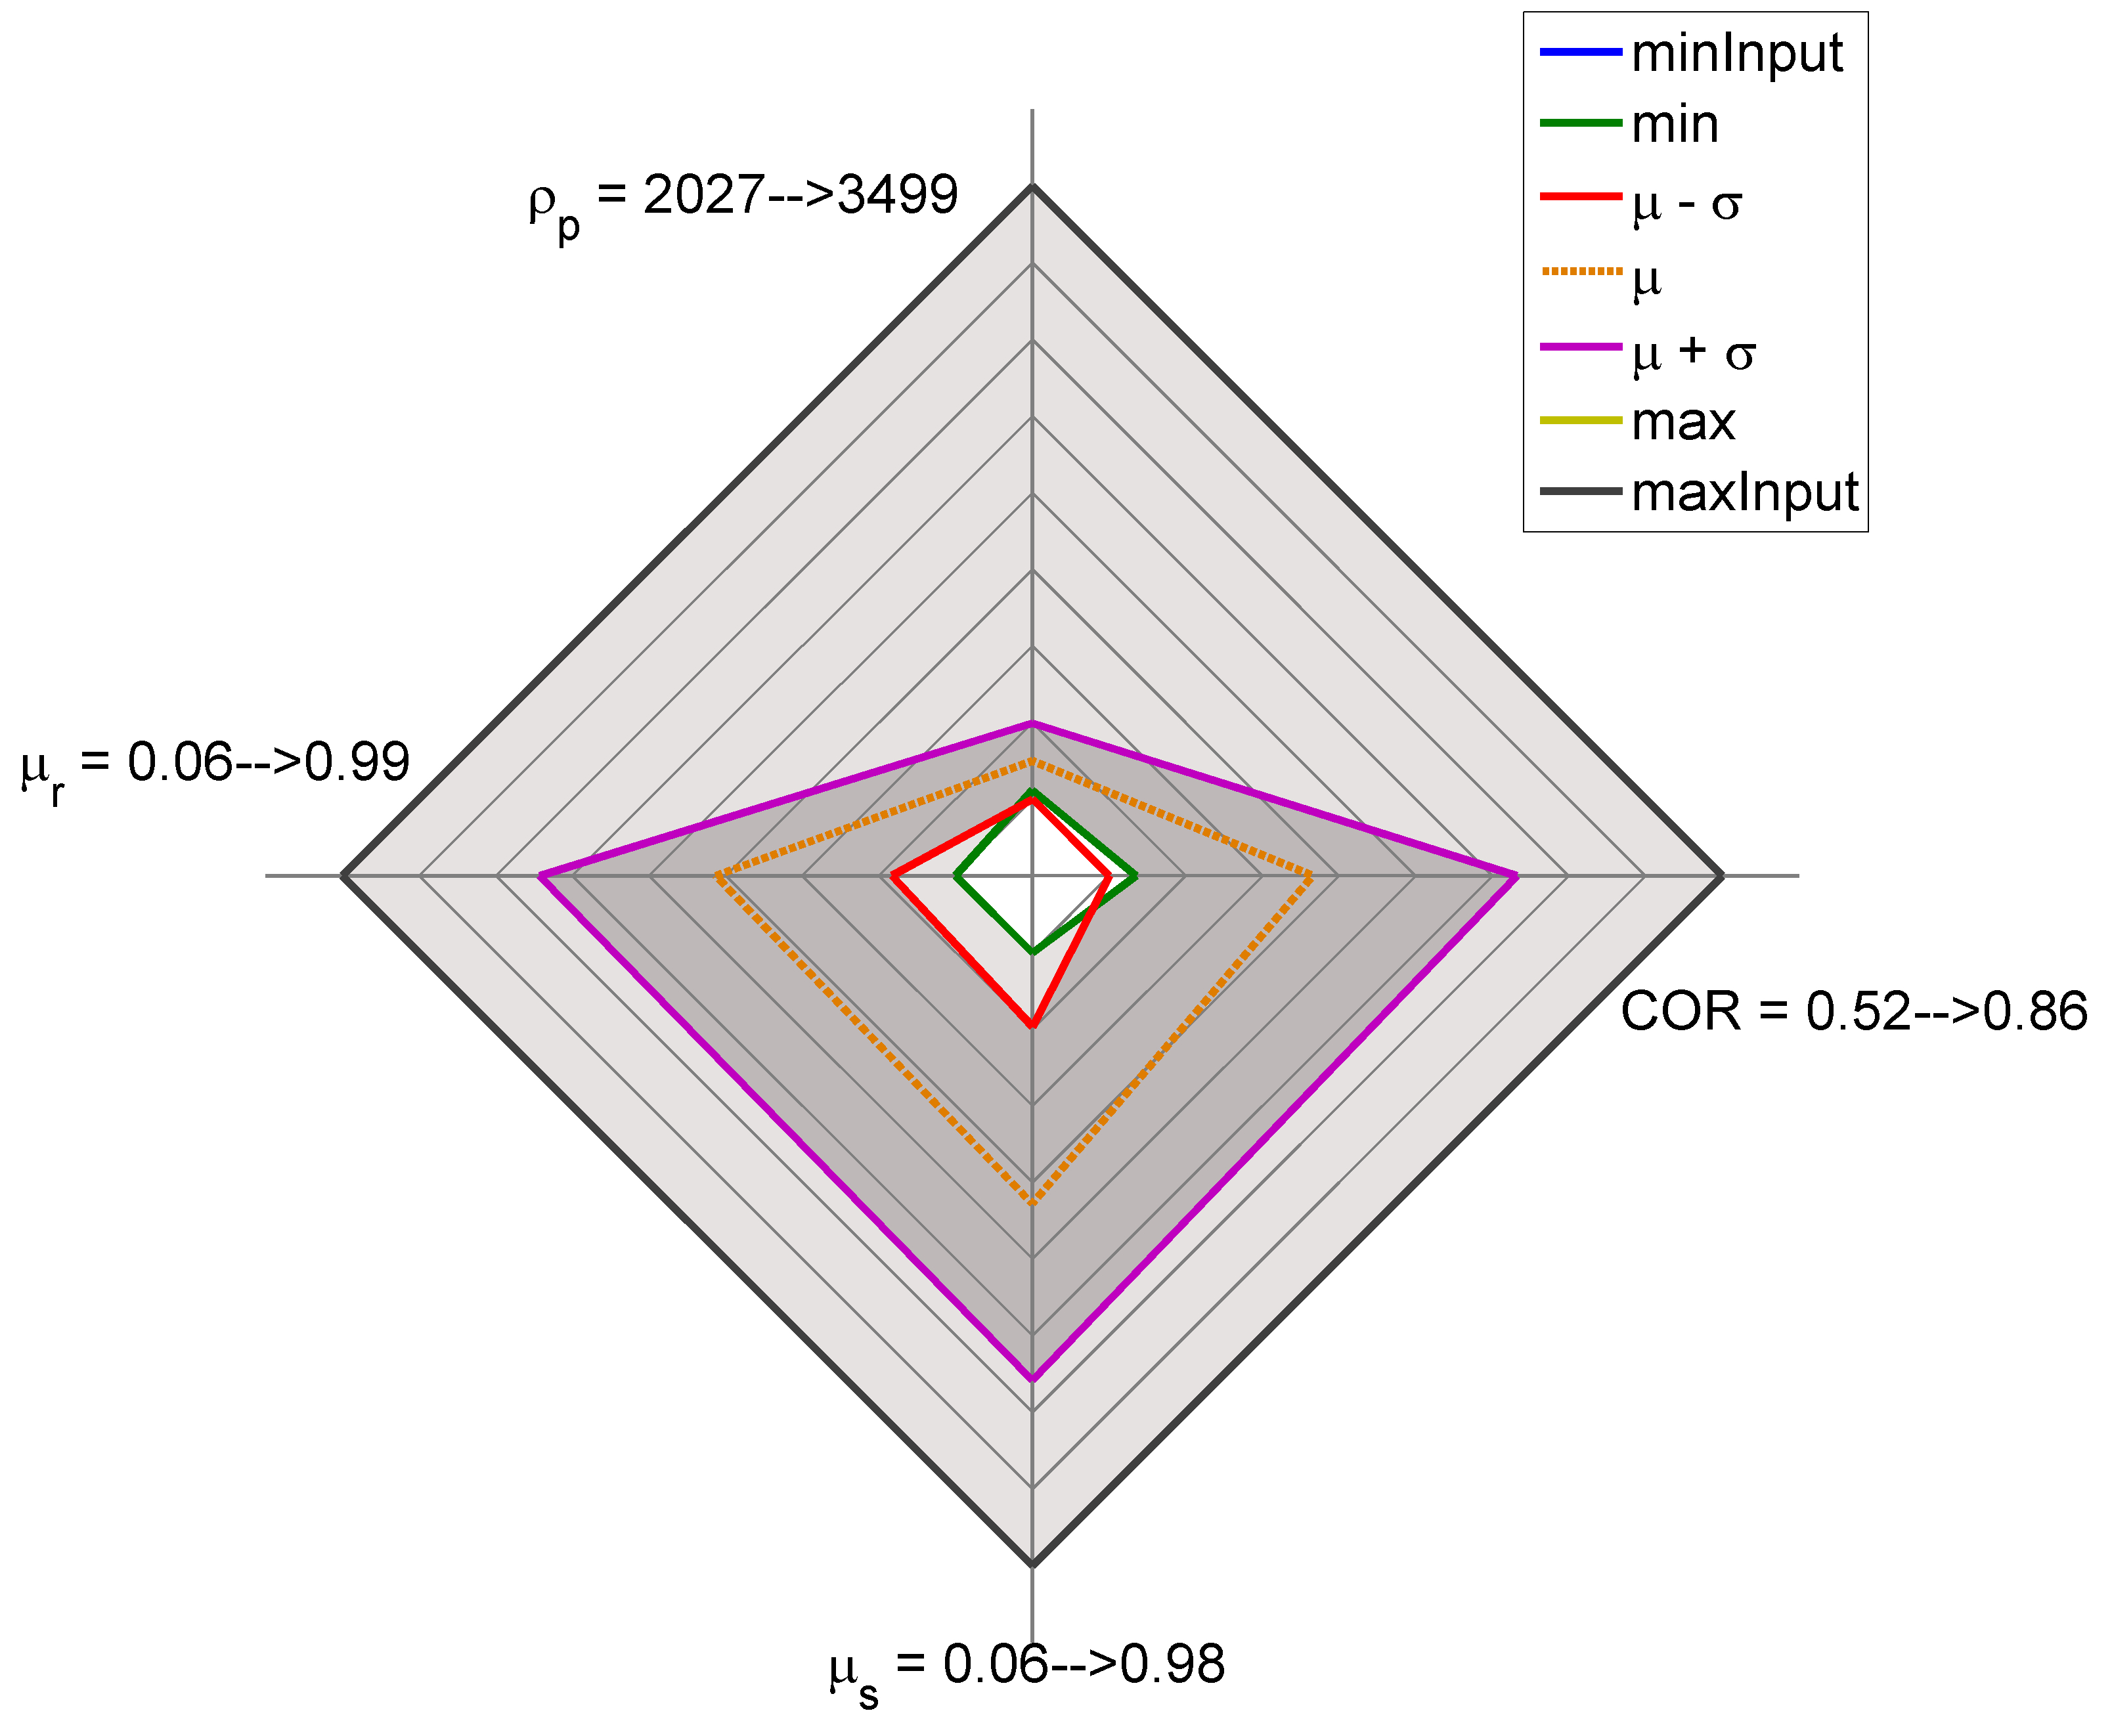
\includegraphics[width=.48\columnwidth]{images/041radarpirker1schulze1068} 
\caption{Parameter space plot, $SSC$, $\sigma_n=1068$ Pa, P=1.0}
\label{fig:041radarpirker1schulze1068} 
\end{figure}
%************************************************
\begin{figure}%[!htb] 
\centering 
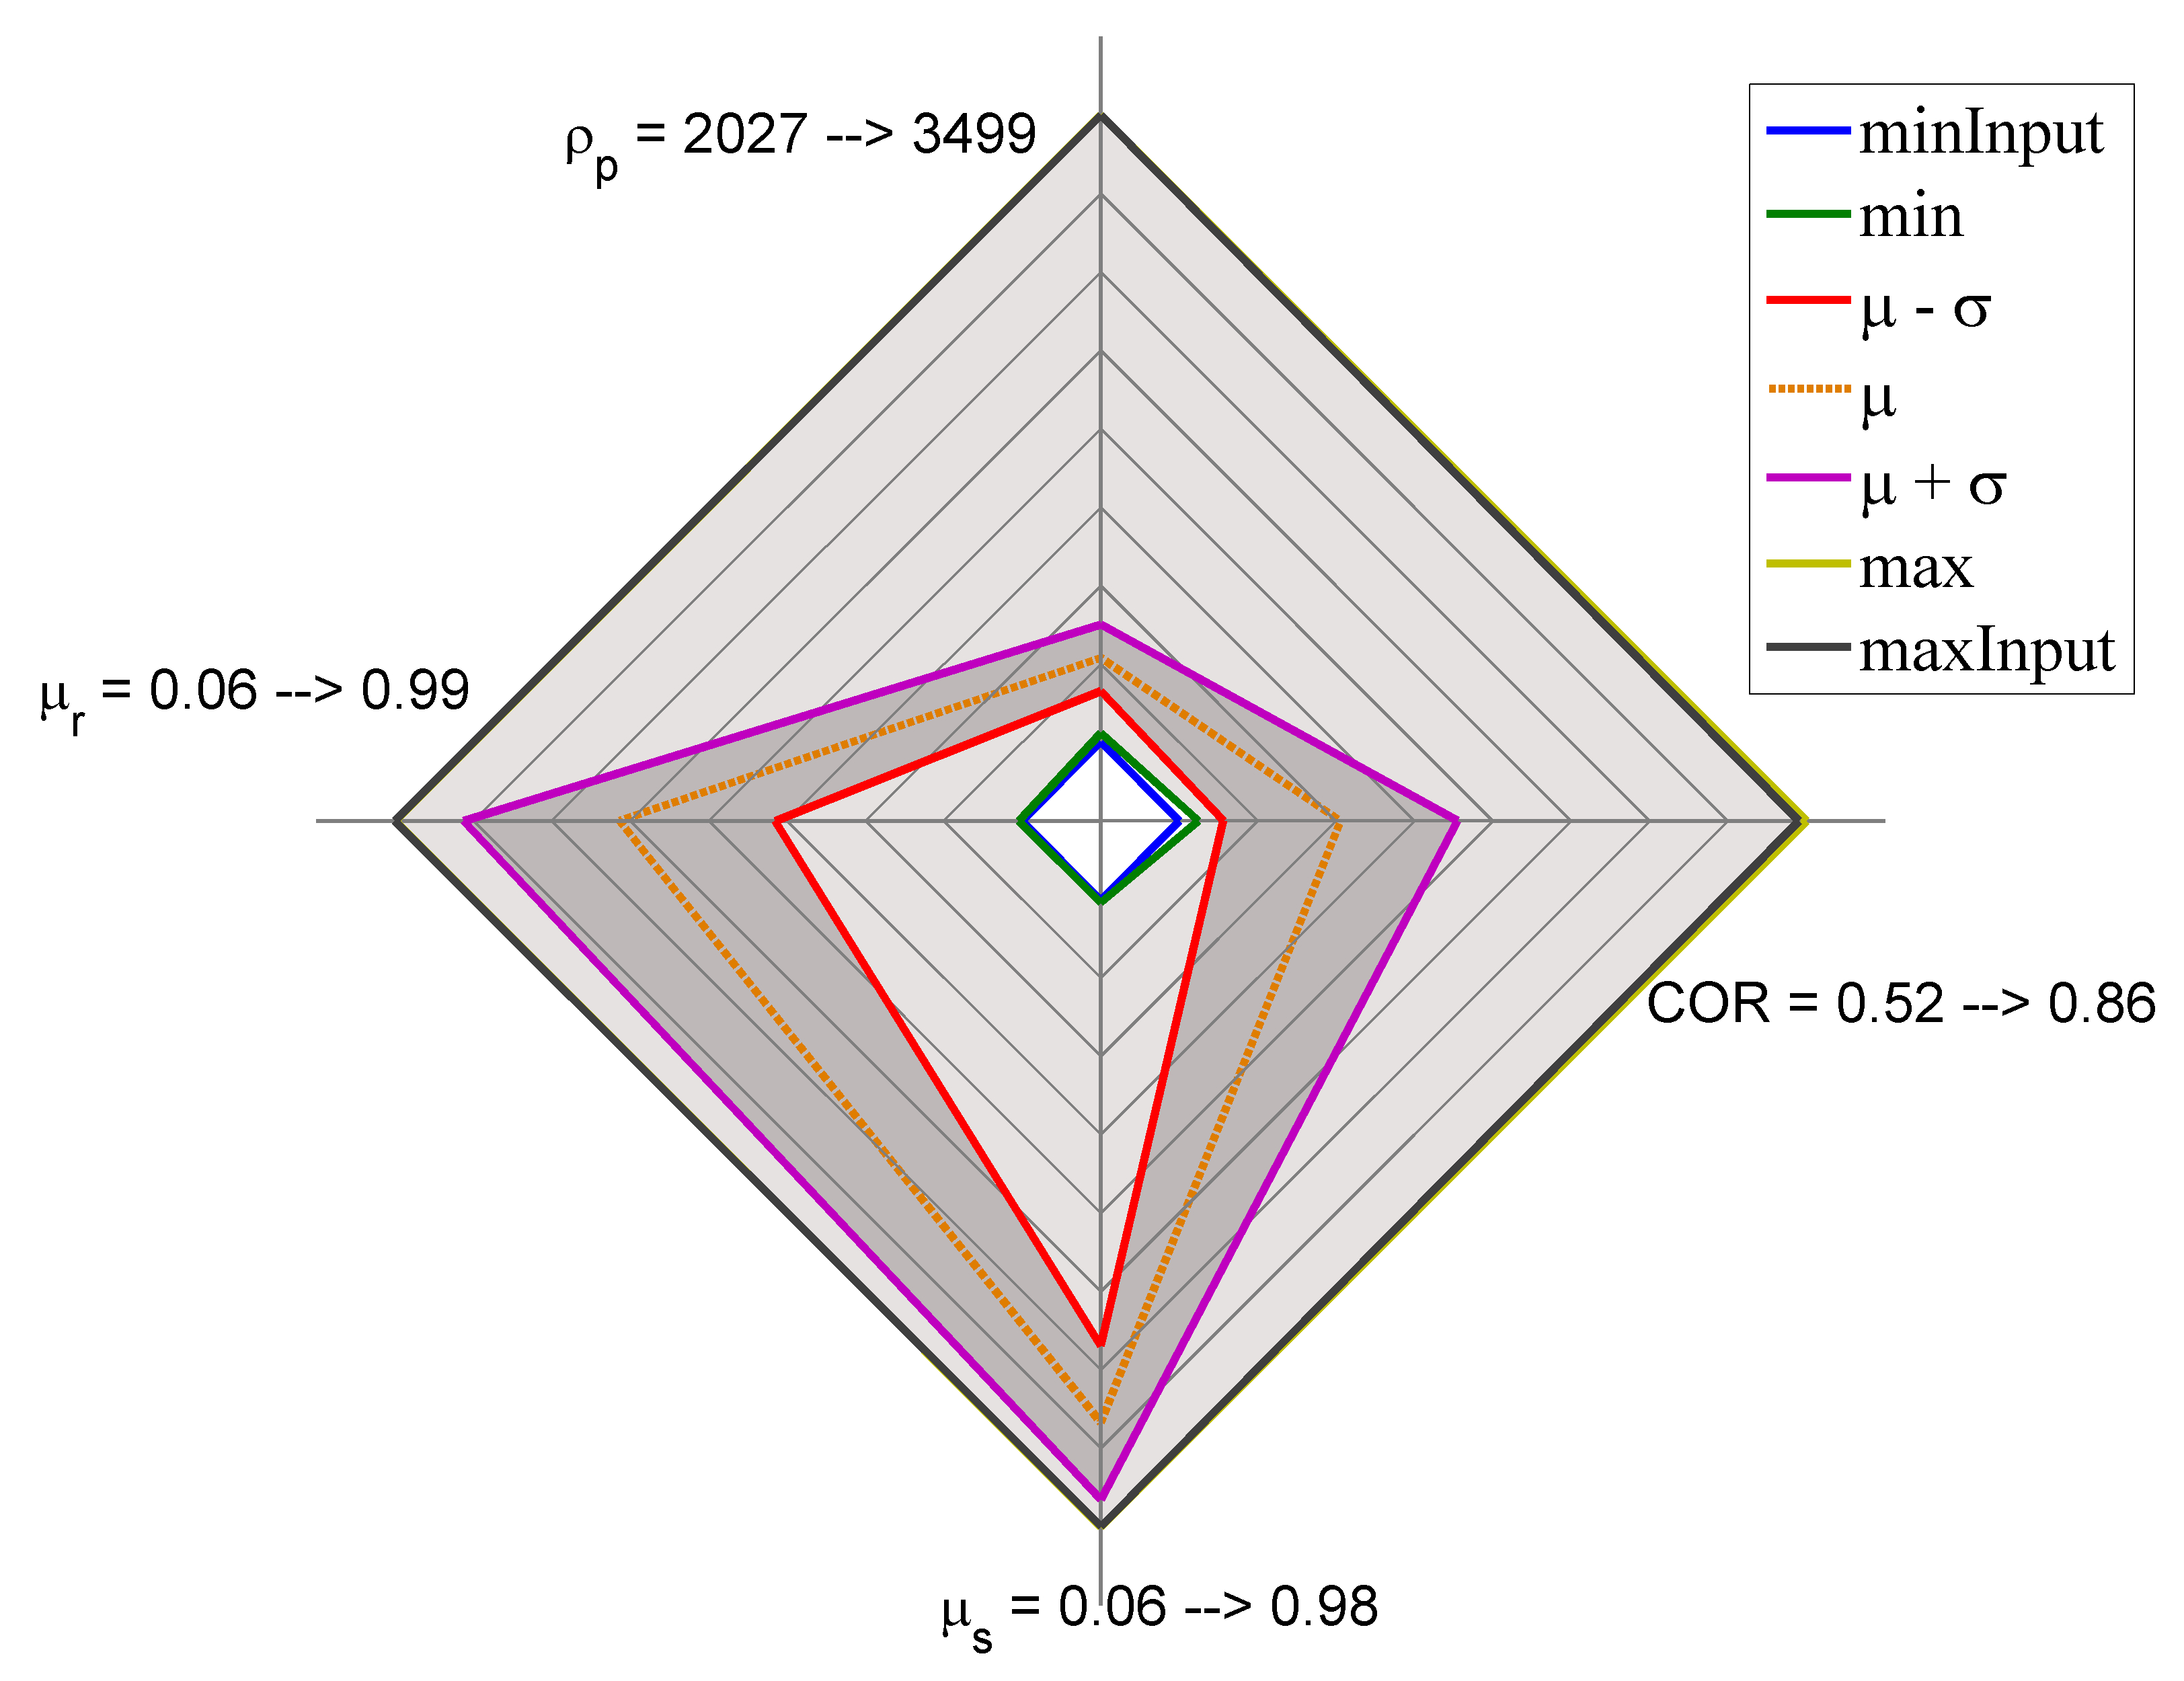
\includegraphics[width=.48\columnwidth]{images/026radarpirker08schulze10070} 
\caption{Parameter space plot, $SSC$, $\sigma_n=10070$ Pa, P=0.8}
\label{fig:026radarpirker08schulze10070} 
\end{figure}
%************************************************
\begin{figure}%[!htb] 
\centering 
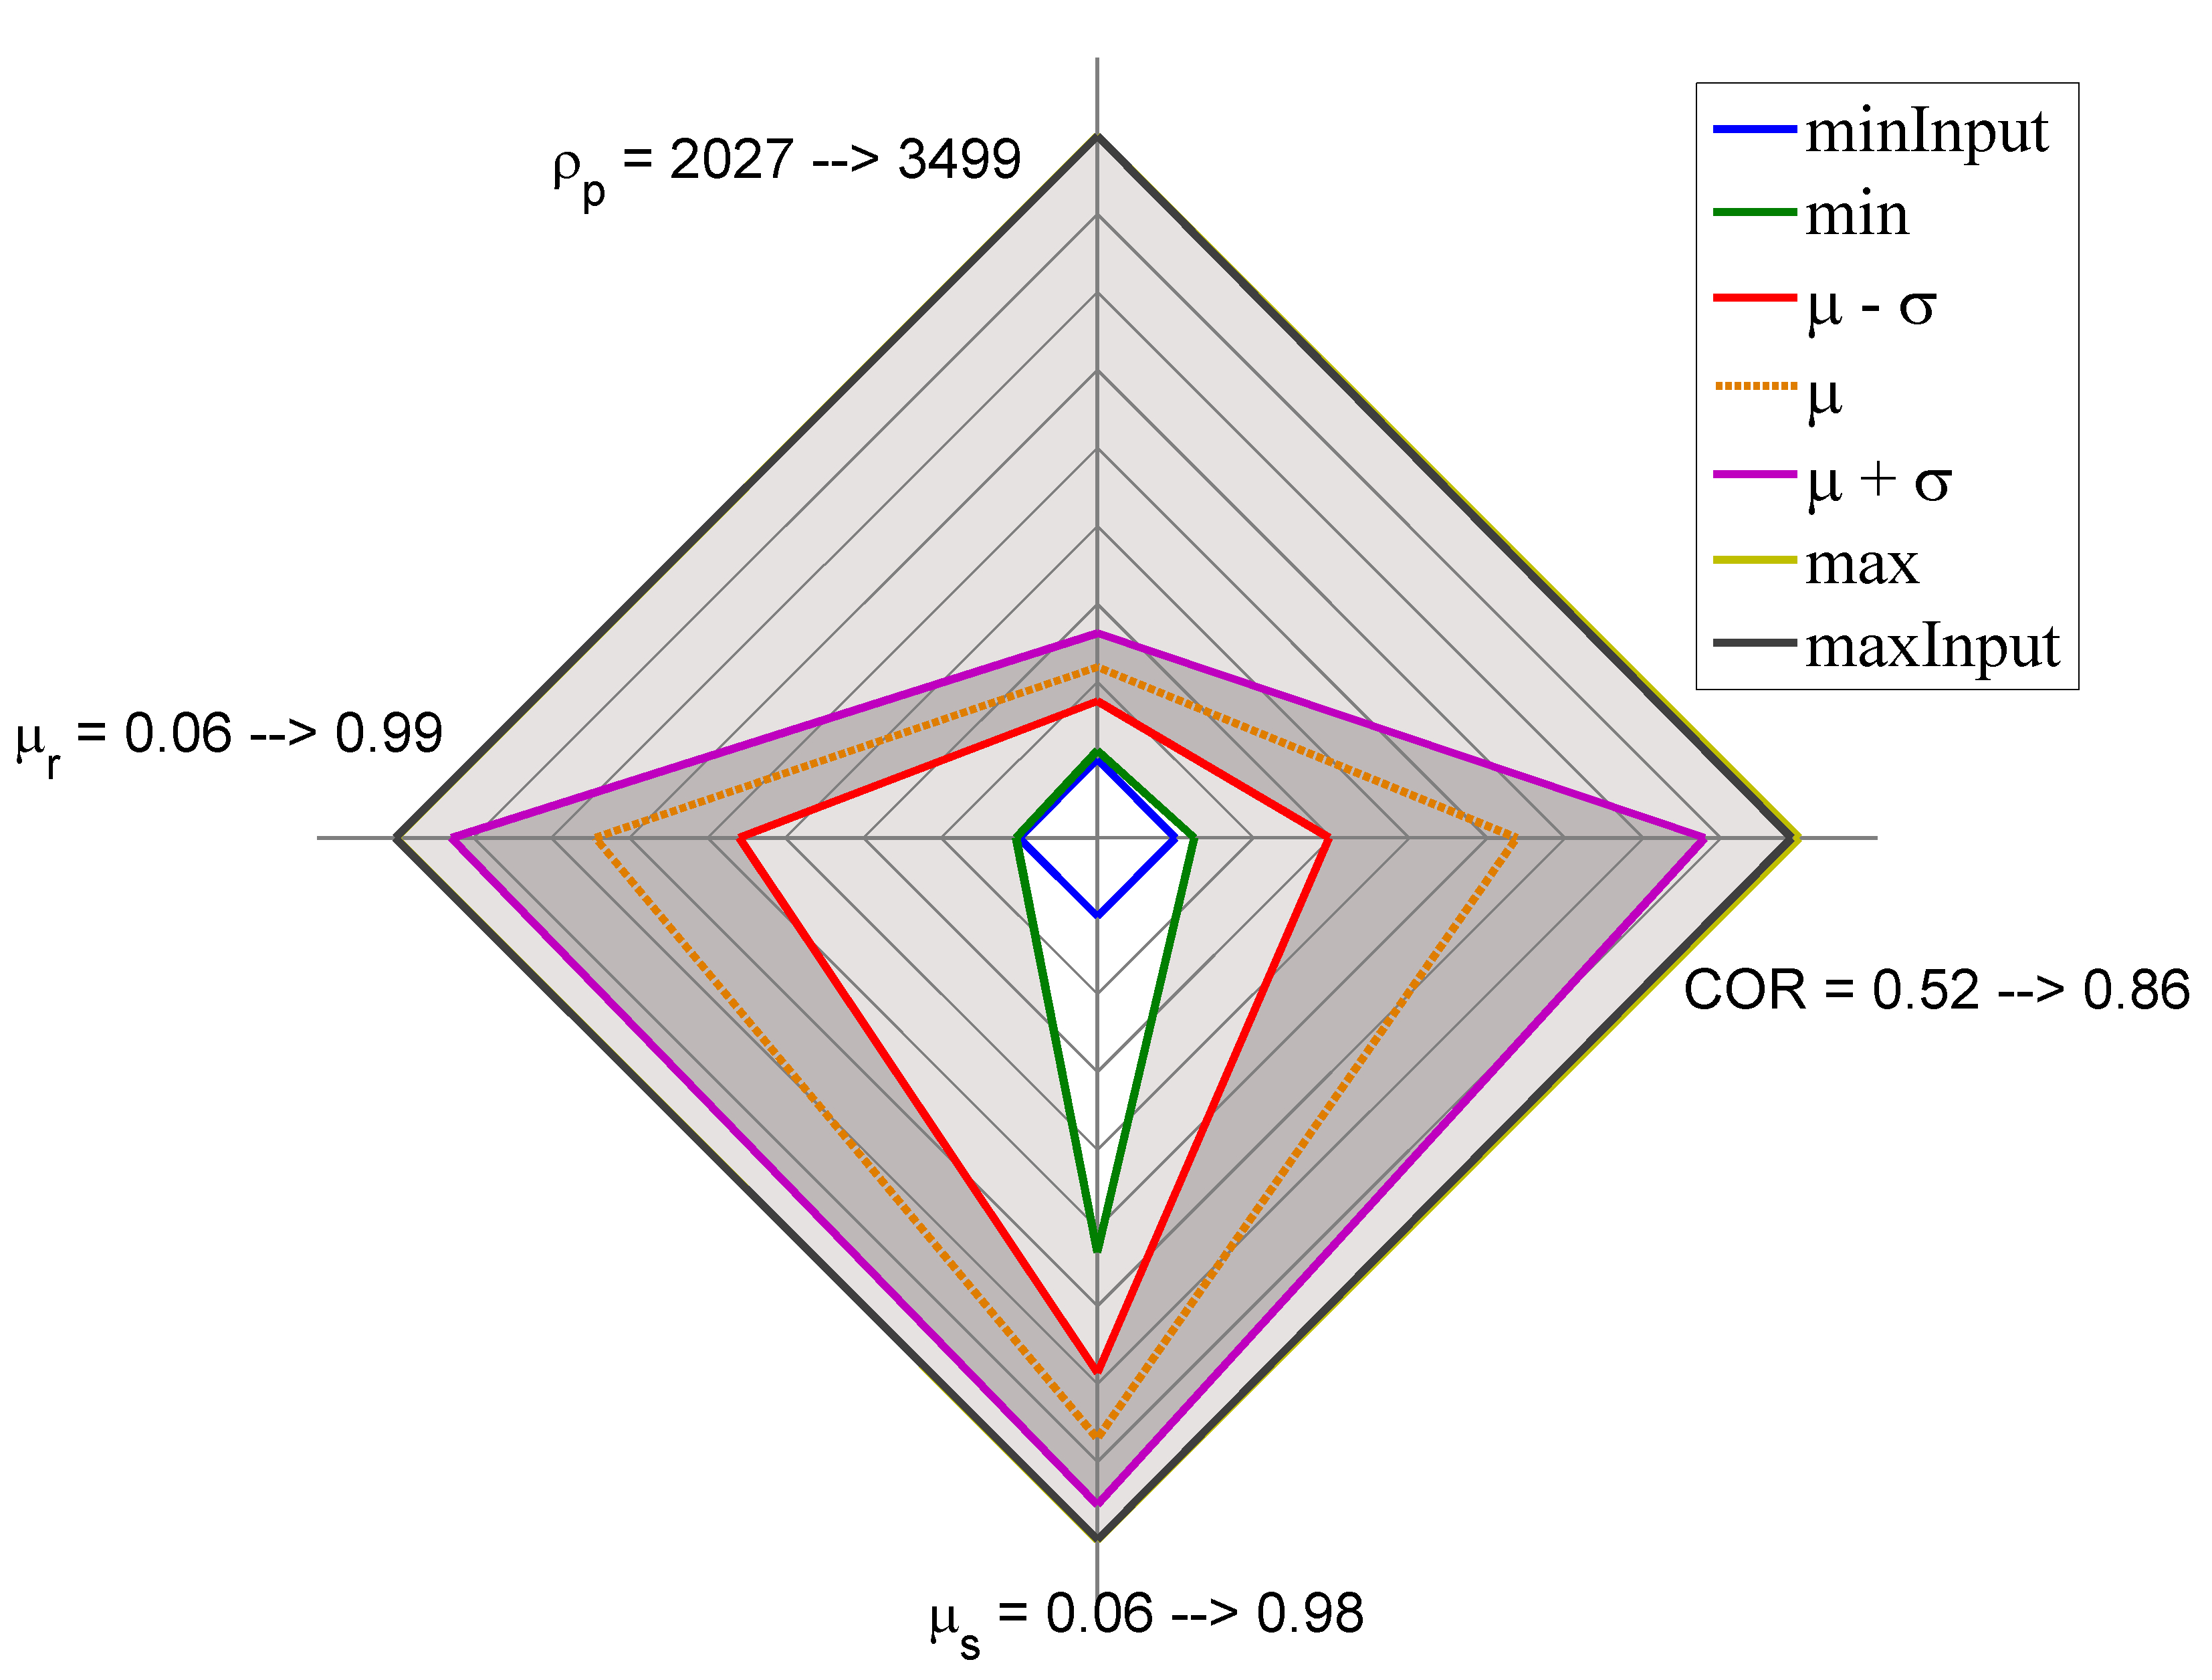
\includegraphics[width=.48\columnwidth]{images/024radarpirker1schulze10070} 
\caption{Parameter space plot, $SSC$, $\sigma_n=10070$ Pa, P=1.0}
\label{fig:024radarpirker1schulze10070} 
\end{figure}
%************************************************
\begin{figure}%[!htb] 
\centering 
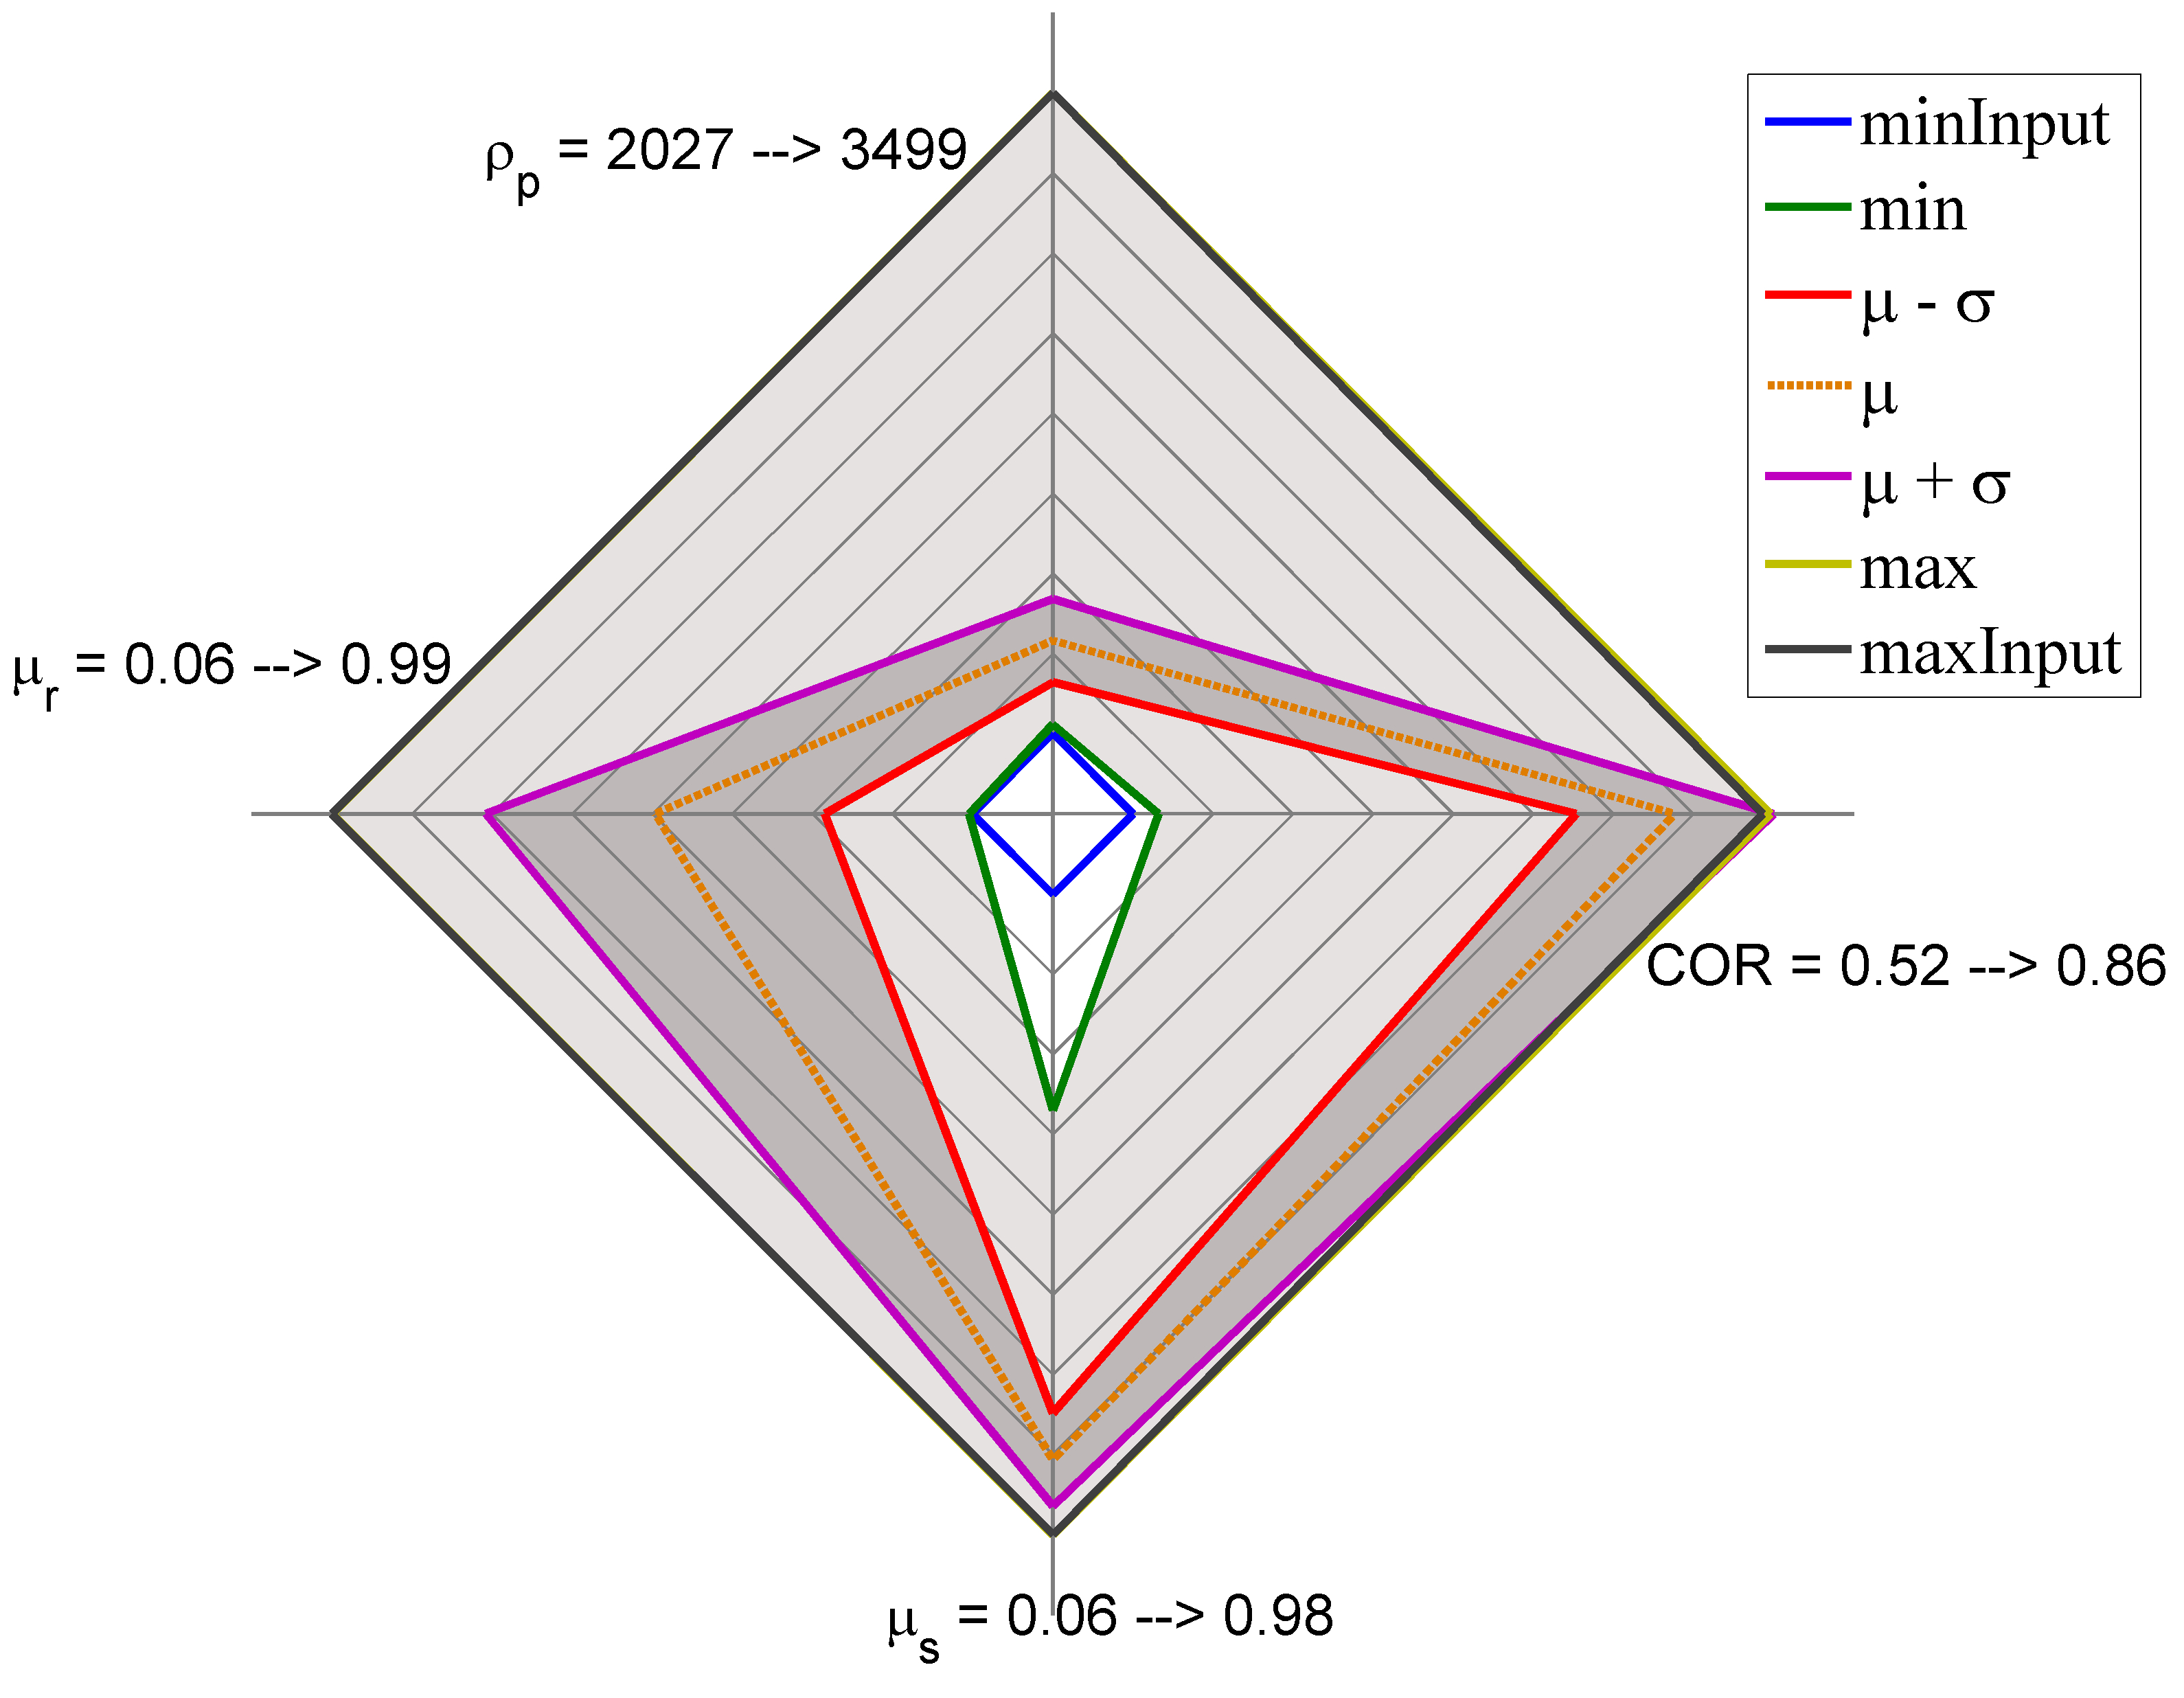
\includegraphics[width=.48\columnwidth]{images/028radarpirker12schulze10070} 
\caption{Parameter space plot, $SSC$, $\sigma_n=10070$ Pa, P=1.2}
\label{fig:028radarpirker12schulze10070} 
\end{figure}
%************************************************
\begin{figure}%[!htb] 
\centering 
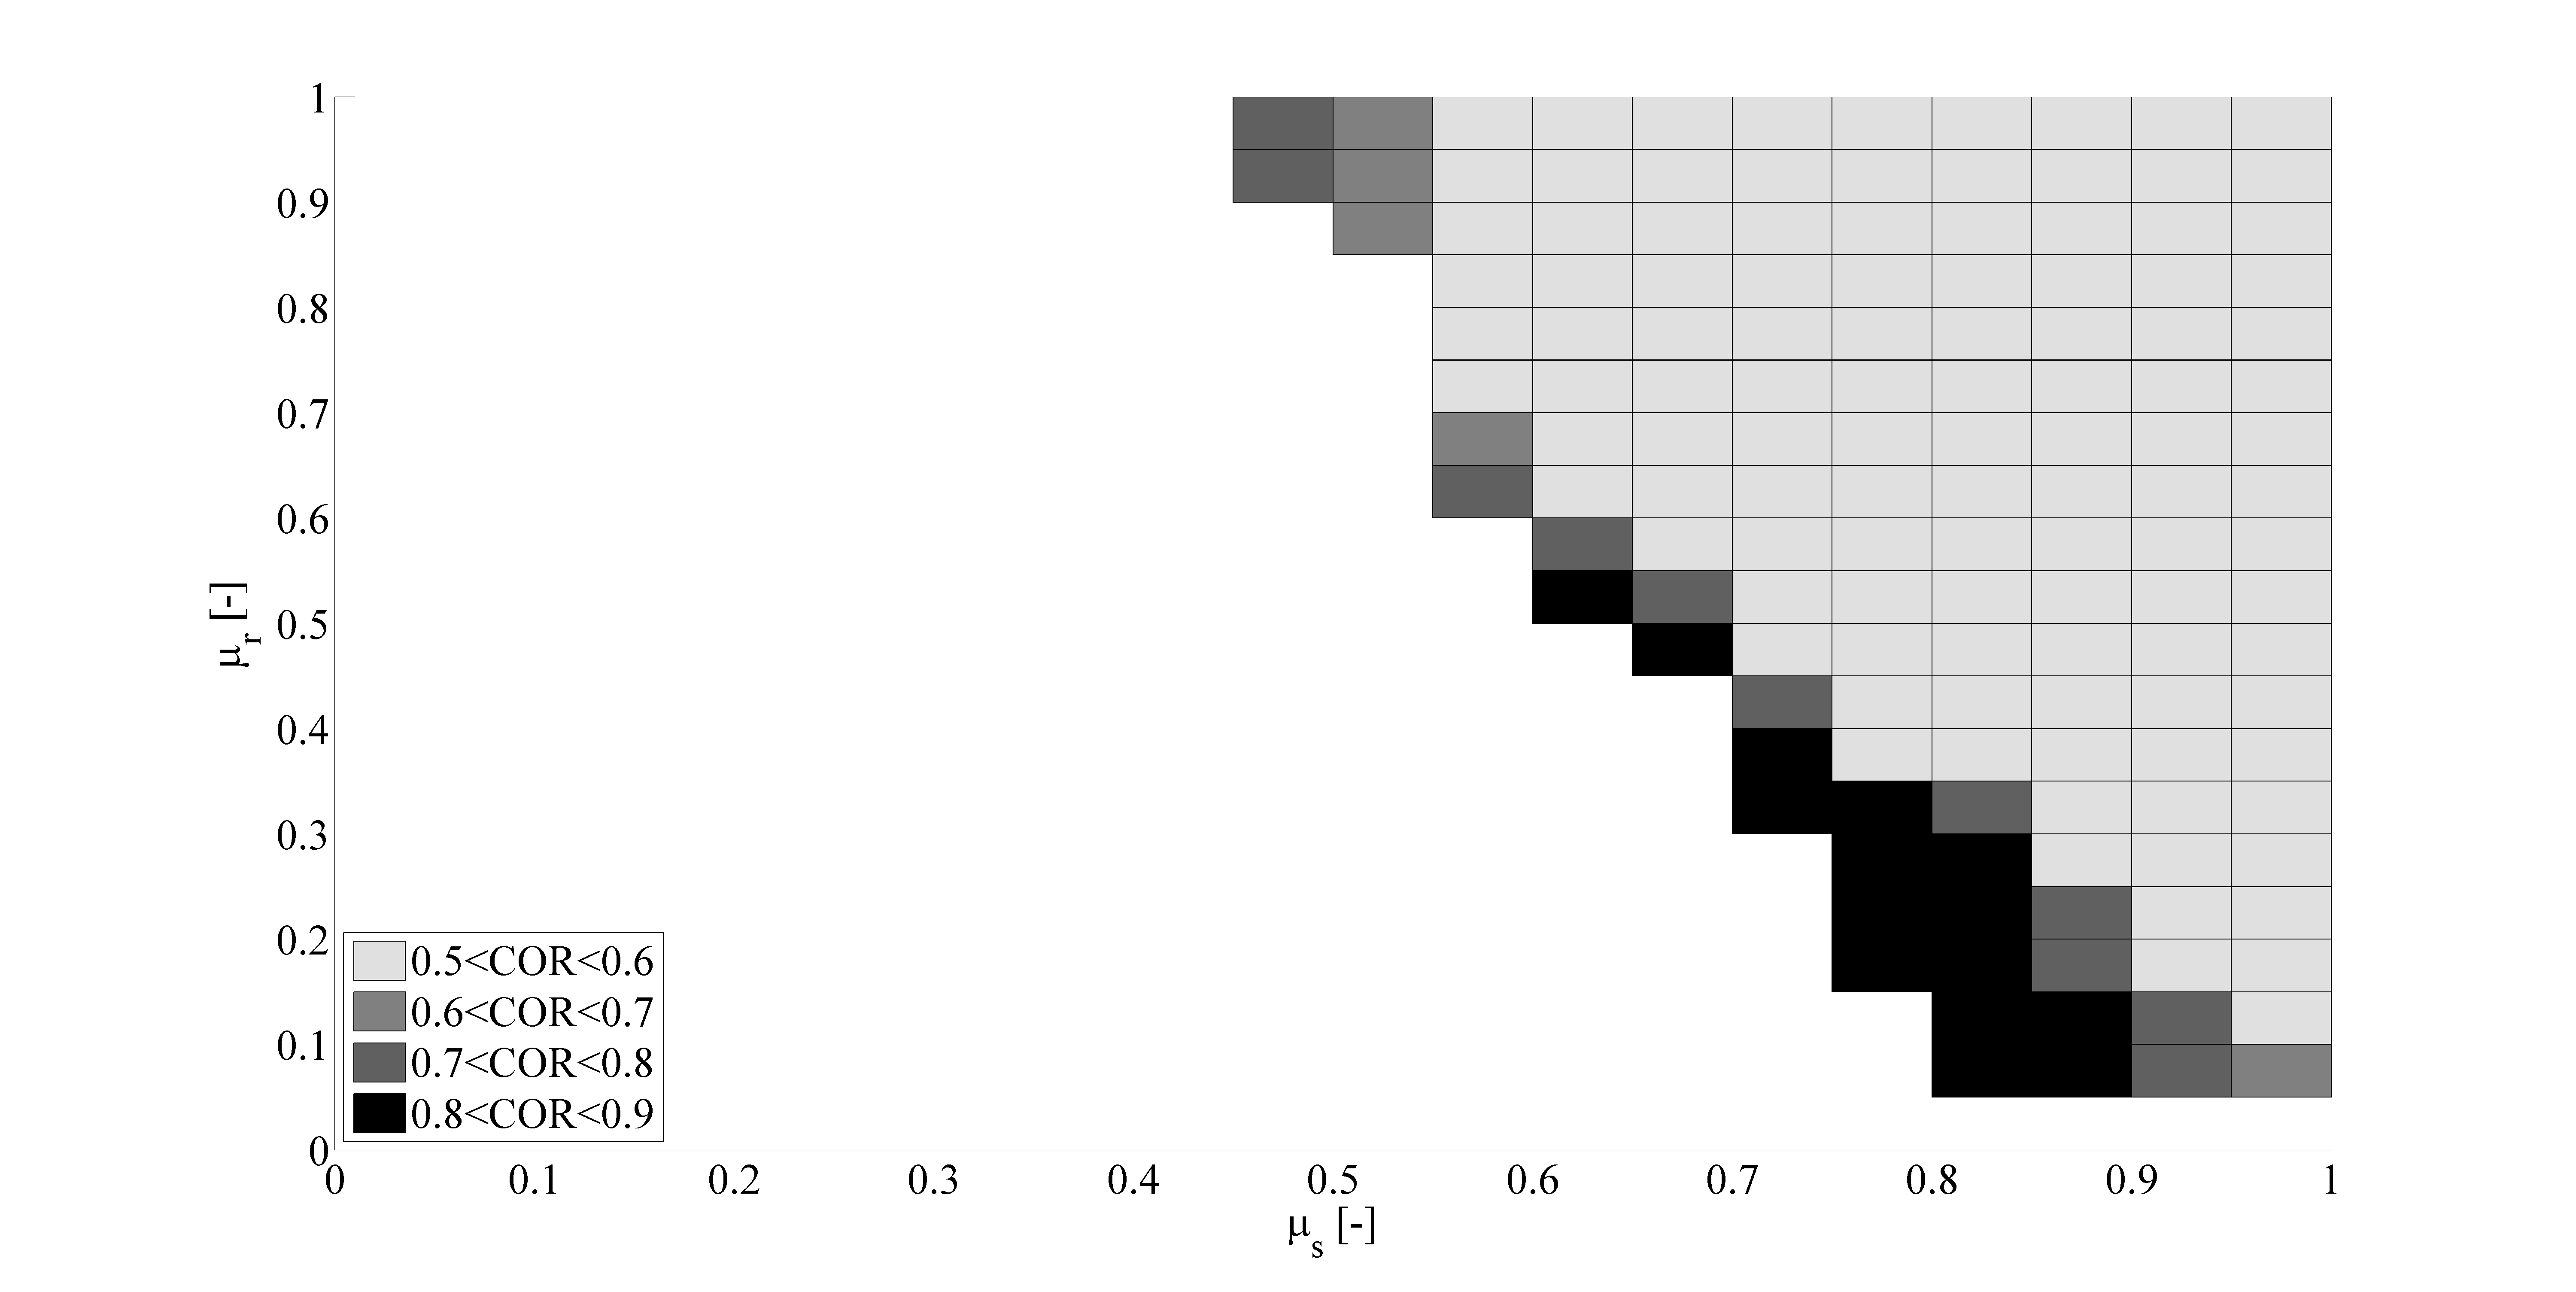
\includegraphics[width=.48\columnwidth]{images/027cloudpirker08schulze10070} 
\caption{Density plot, $SSC$, $\sigma_n=10070$ Pa, P=0.8}
\label{fig:027cloudpirker08schulze10070} 
\end{figure}
%************************************************
\begin{figure}%[!htb] 
\centering 
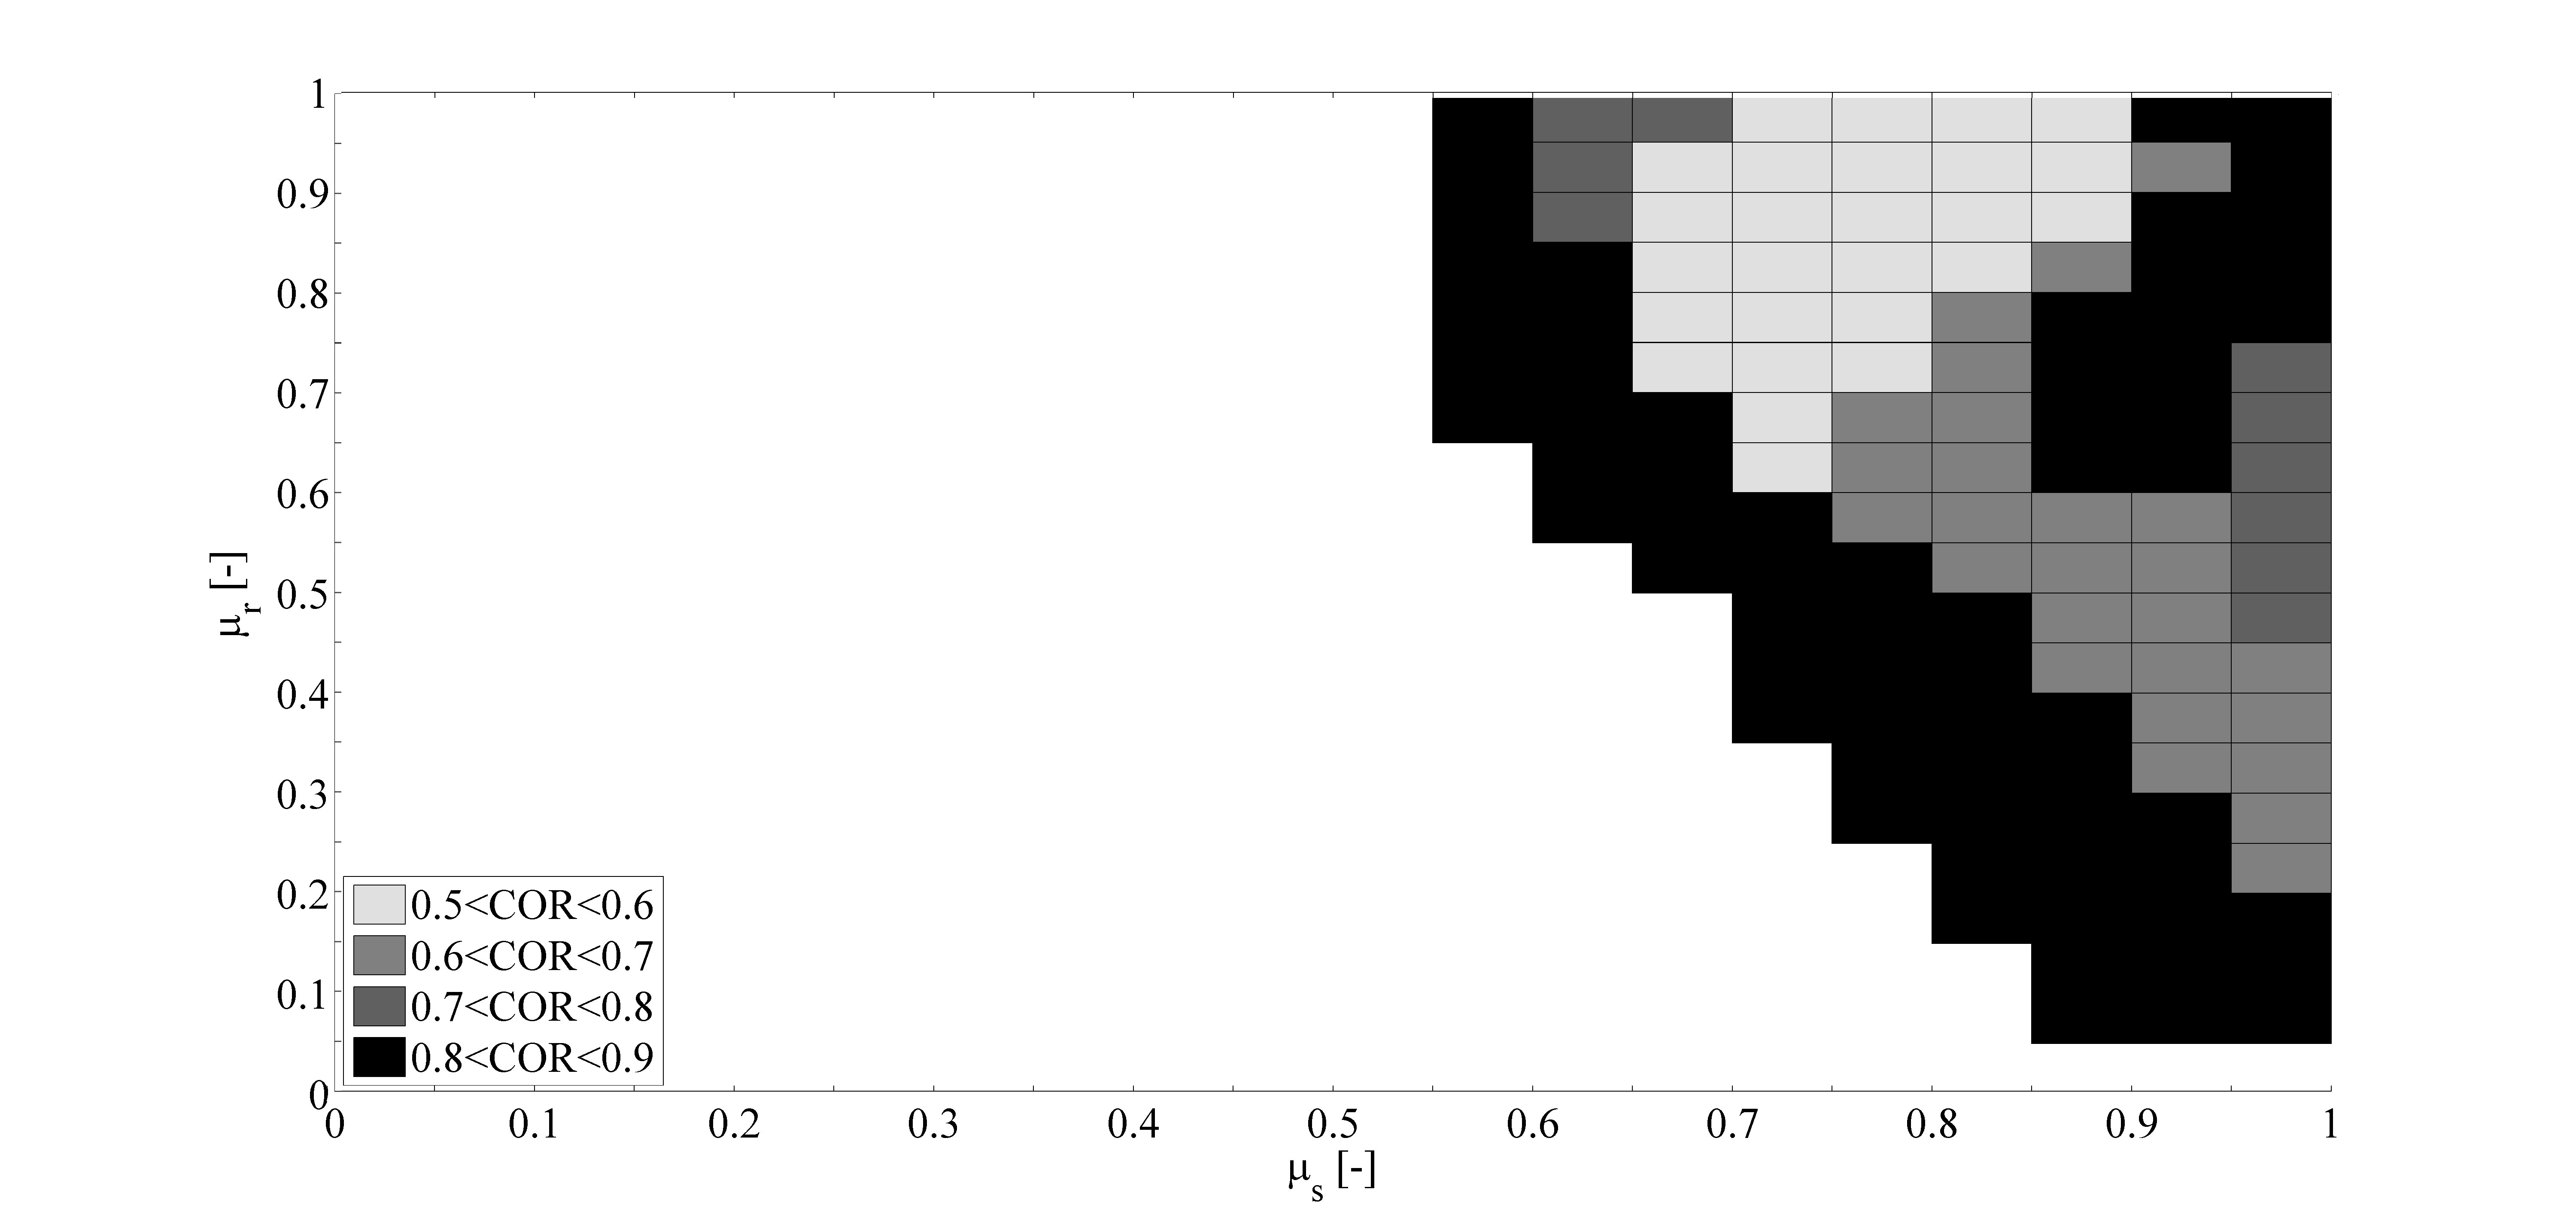
\includegraphics[width=.48\columnwidth]{images/025cloudpirker1schulze10070} 
\caption{Density plot, $SSC$, $\sigma_n=10070$ Pa, P=1.0}
\label{fig:025cloudpirker1schulze10070} 
\end{figure}
%************************************************
\begin{figure}%[!htb] 
\centering 
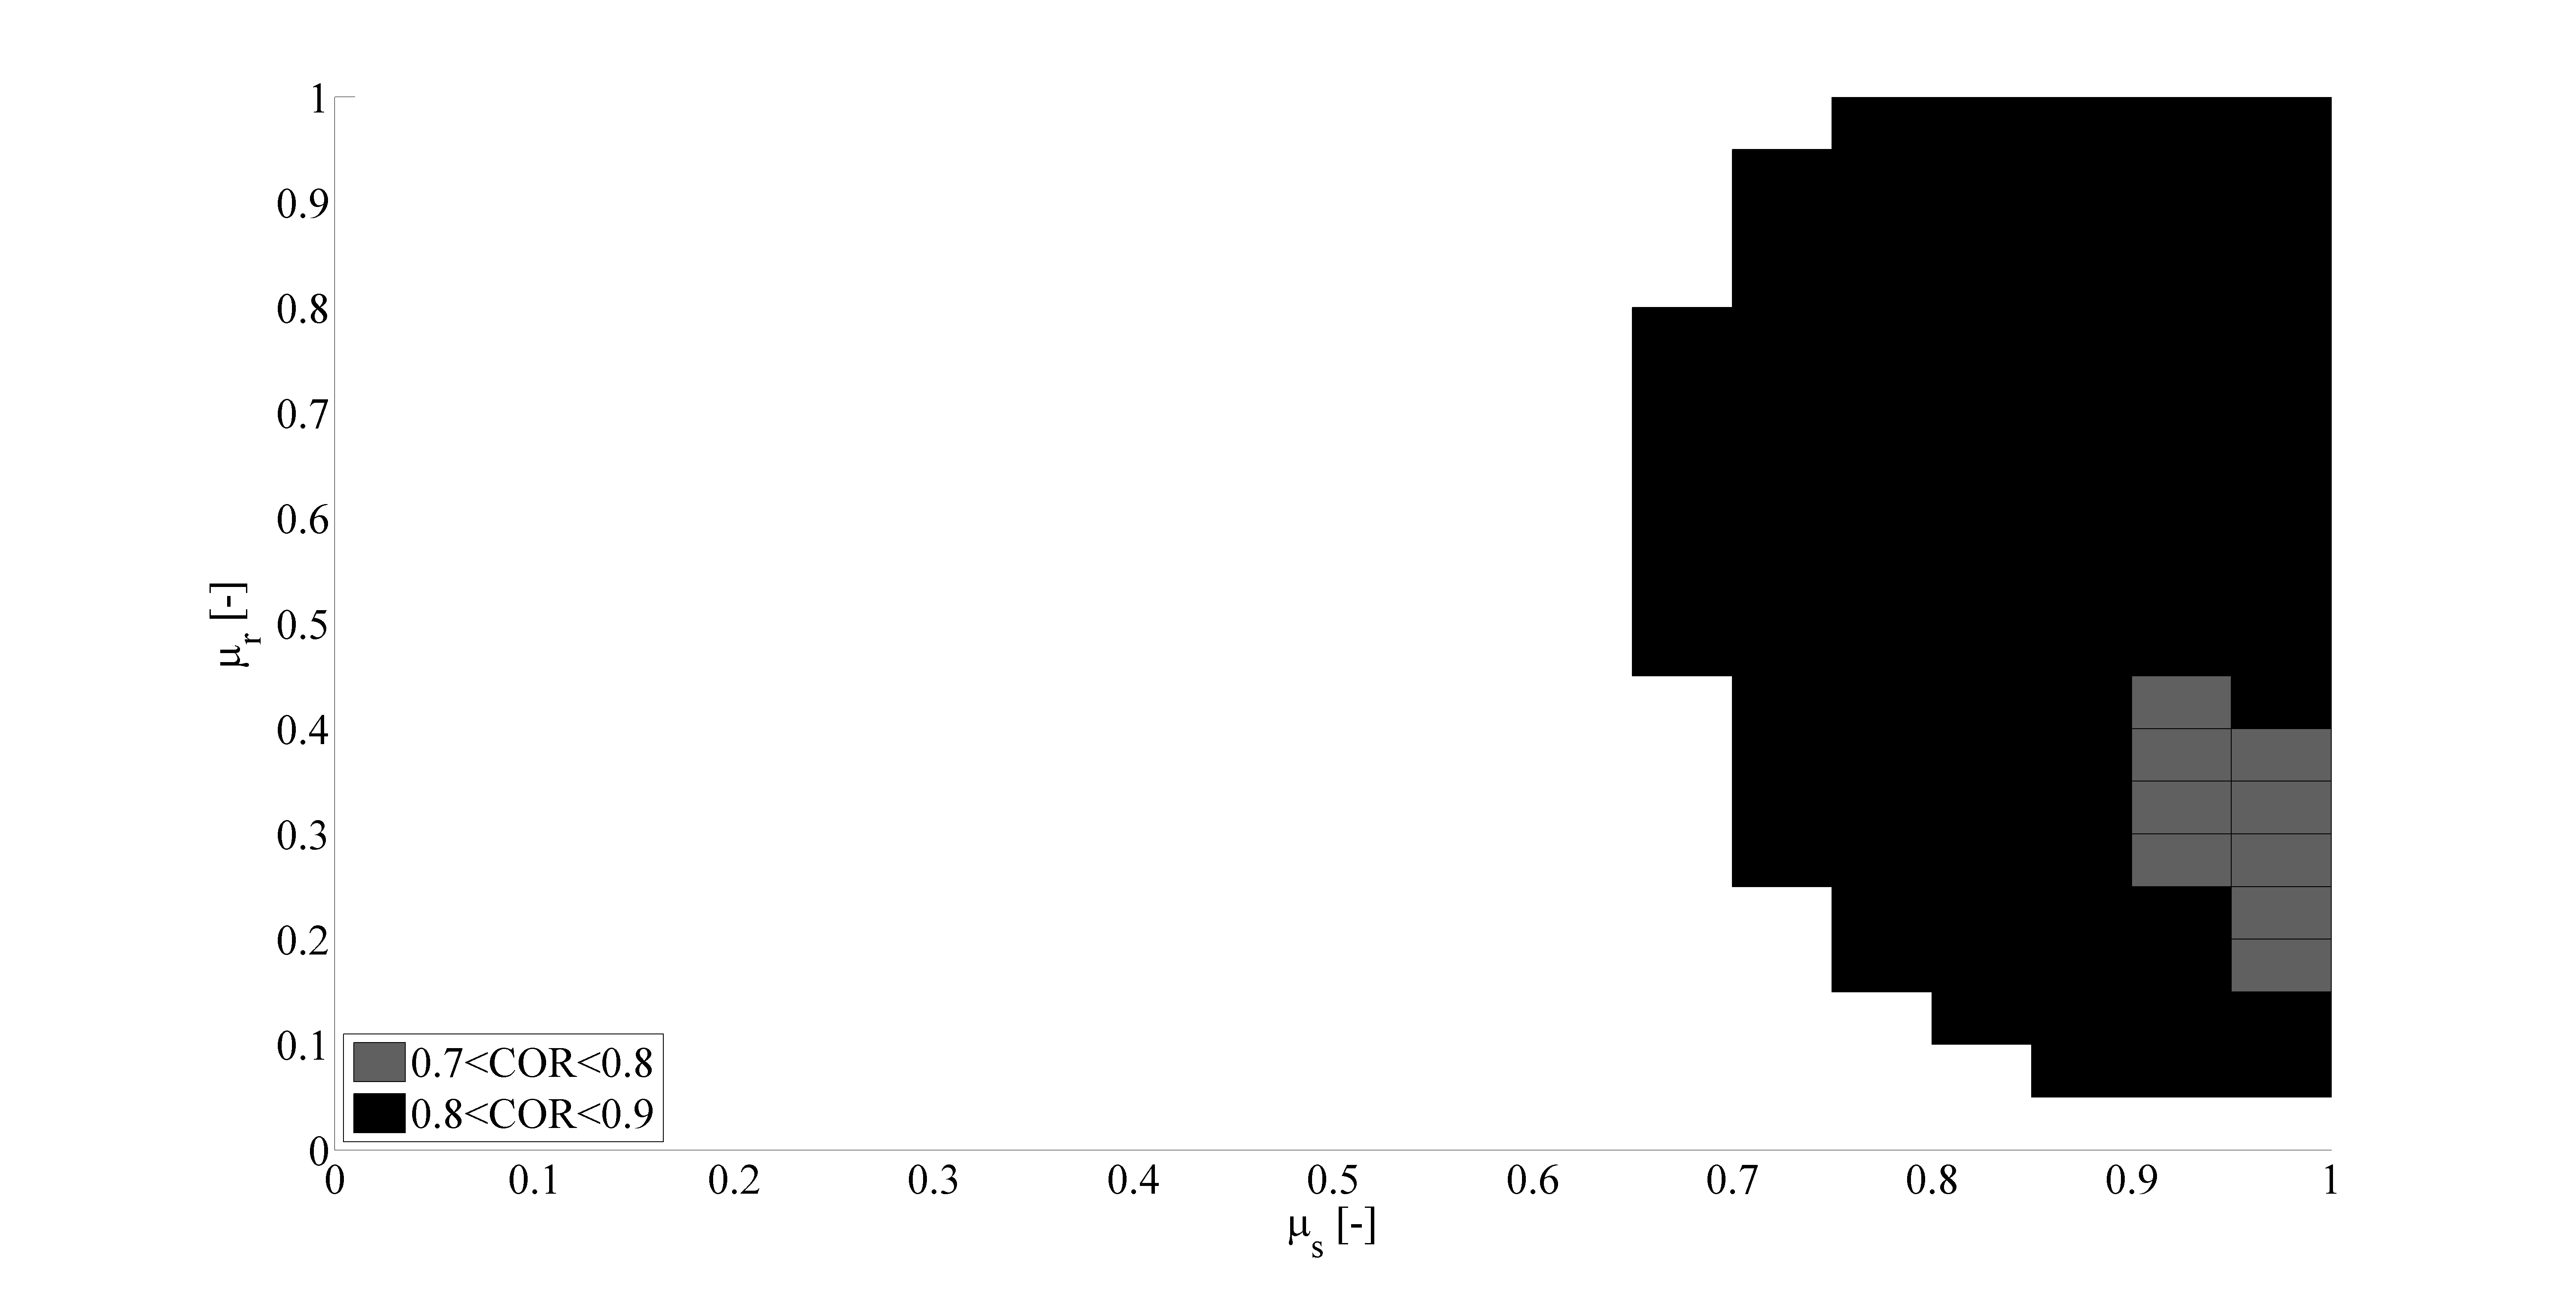
\includegraphics[width=.48\columnwidth]{images/030cloudpirker12schulze10070} 
\caption{Density plot, $SSC$, $\sigma_n=10070$ Pa, P=1.2}
\label{fig:030cloudpirker12schulze10070} 
\end{figure}
%************************************************

\begin{figure}%[!htb] 
\centering 
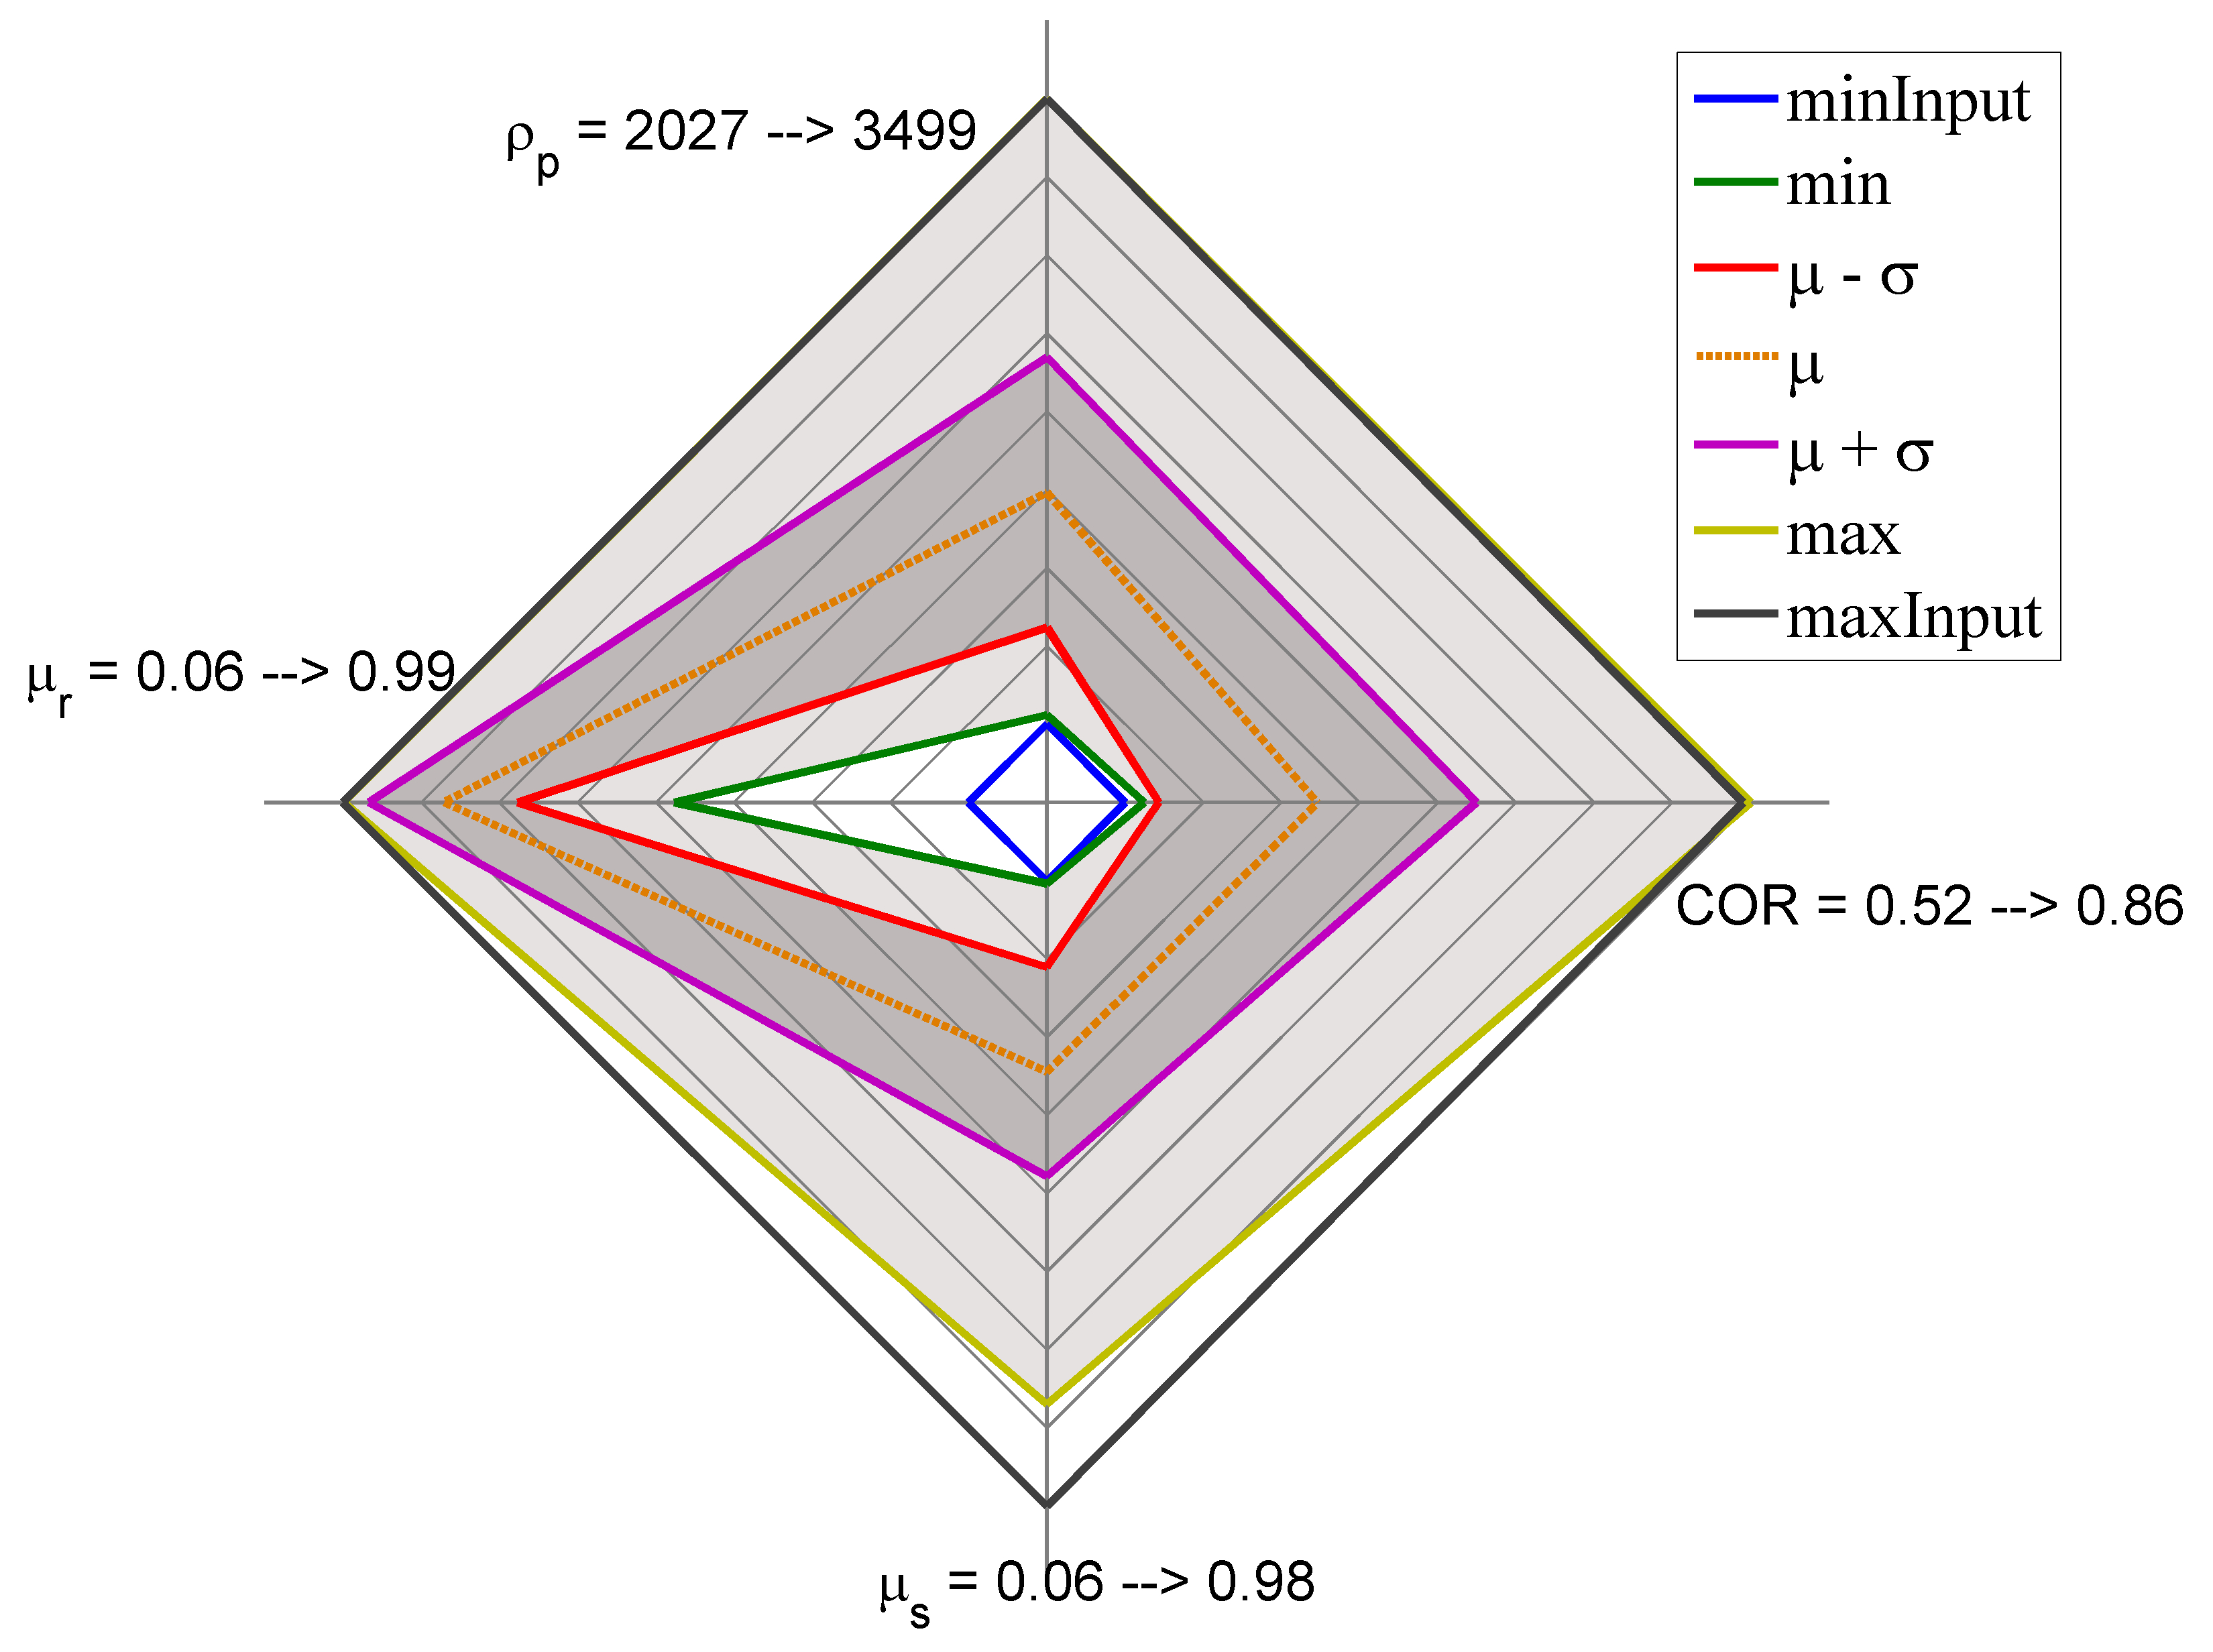
\includegraphics[width=.48\columnwidth]{images/031radarpirker1aor} 
\caption{Parameter space plot, $AoR_{exp} = 38.85 ^\circ$}
\label{fig:031radarpirker1aor} 
\end{figure}
%************************************************
\begin{figure}%[!htb] 
\centering 
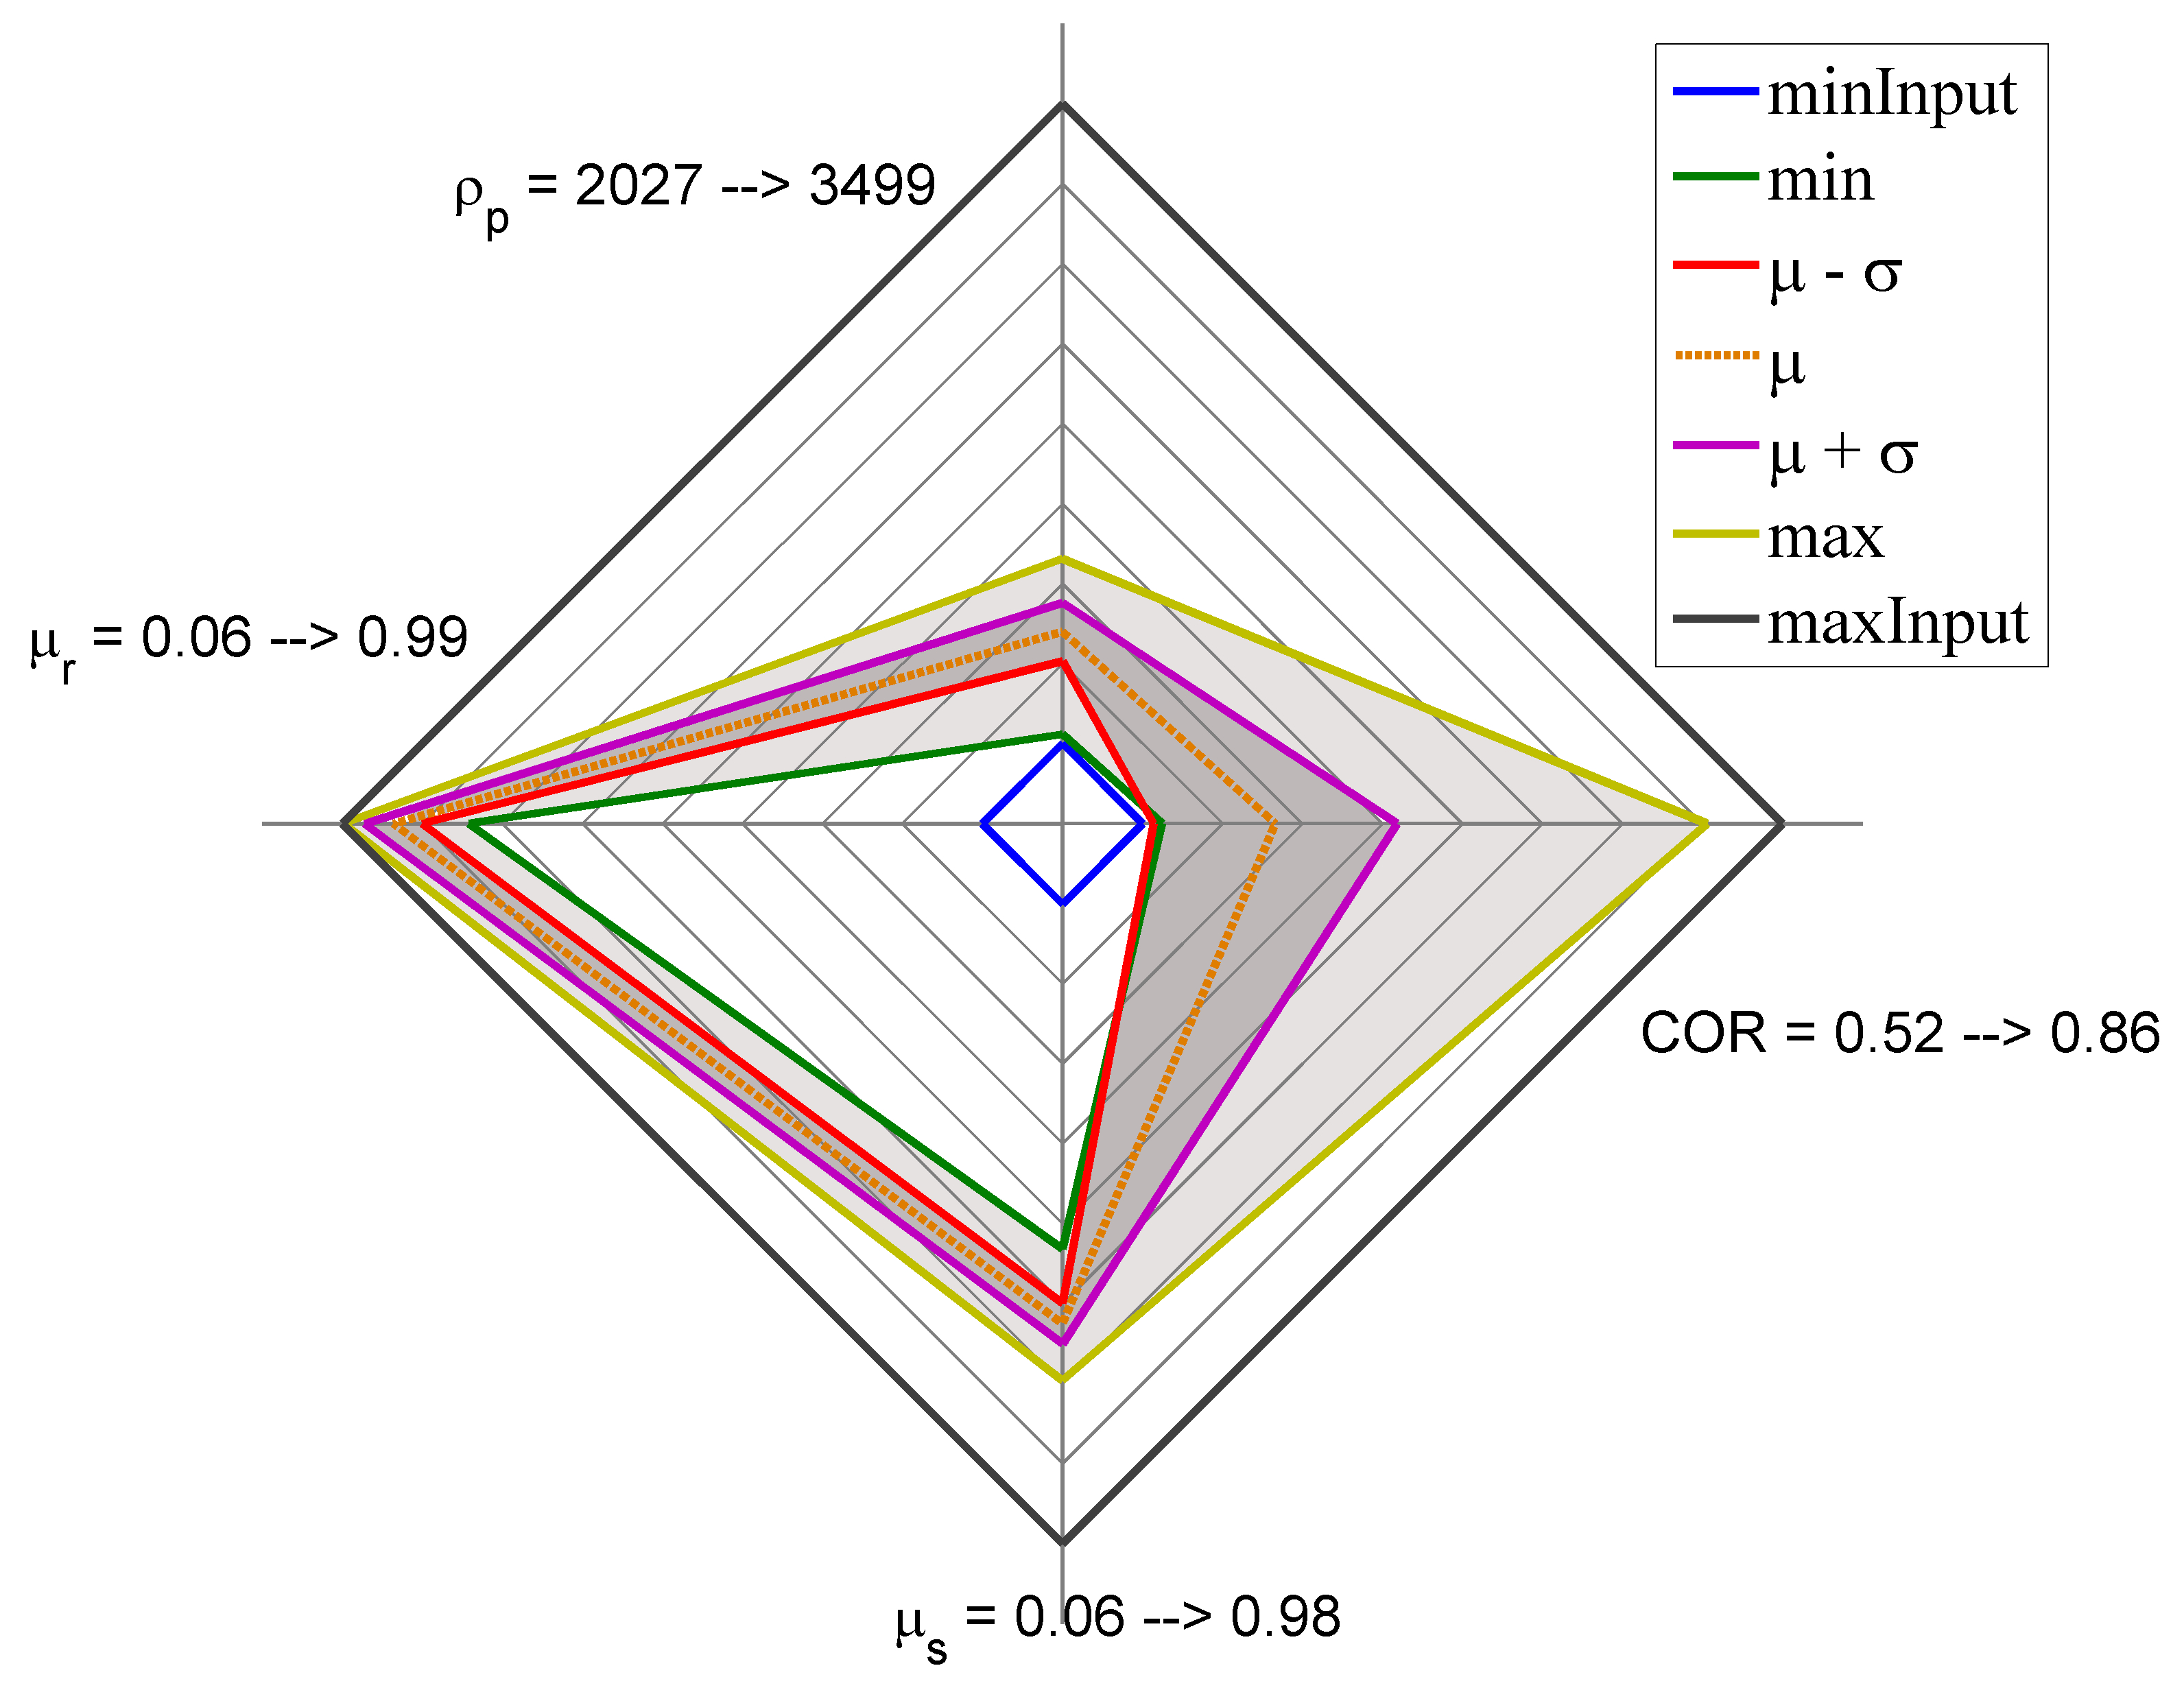
\includegraphics[width=.48\columnwidth]{images/033radarpirker1schulze10070aor} 
\caption{Parameter space plot, $AoR_{exp} = 38.85
        ^\circ$ \& $SSC$: $\sigma_n=10070$ Pa}
\label{fig:033radarpirker1schulze10070aor} 
\end{figure}
%************************************************